%%%%%%%%%%%%%%%%%%%%%%%%%%%%%%%%%%%%%%%%%%%%%%%%%%%%%%%%%%%%%%%%%%%%%%%%
%                                                                      %
%     File: Thesis_Results.tex                                         %
%     Tex Master: Thesis.tex                                           %
%                                                                      %
%     Author: Andre C. Marta                                           %
%     Last modified :  2 Jul 2015                                      %
%                                                                      %
%%%%%%%%%%%%%%%%%%%%%%%%%%%%%%%%%%%%%%%%%%%%%%%%%%%%%%%%%%%%%%%%%%%%%%%%

\chapter{Results}
\label{chapter:results}

In this chapter we describe the main results of the search for $hh\rightarrow b\overline{b}b\overline{b}$ at the FCC-hh using two benchmark luminosities, $30~\text{ab}^{-1}$ and $3~\text{ab}^{-1}$ (section \ref{sec:dihiggs_FCC}). The statistical analysis used to extract the signal strength and to set limits on the Higgs boson triple coupling is also discussed. In section \ref{sec:gran_studies} we show how the significance of the analysis varies as a function of the granularity of the HCAL and/or the detector configuration. We also compare the results obtained using particle flow and pure calorimeter jets.

\section{Di-Higgs discovery potential at the FCC-hh}
\label{sec:dihiggs_FCC}

The event selection of the baseline analysis for the search for $hh\rightarrow b\overline{b}b\overline{b}$ at the FCC with the baseline detector design is summarized in tables \ref{table:cutflow_sig_FCC} and \ref{table:cutflow_bkg_FCC} for the signal samples (SM, DM mediator and type II 2HDM) and for the background samples ($4b+j$, $jj+0/1/2 j$ and $t\overline{t}$), respectively.

From table \ref{table:cutflow_sig_FCC}, we see that for the BSM models, the signal efficiency is higher than for the SM. It goes from $0.422$ in the SM, to $0.487$ in the DM mediator model and to $1.342$ in the type II 2HDM.

Considering the SM production of Higgs pairs, the achieved significance is
\begin{equation}
	S/\sqrt{B}=6.8\pm 0.7\quad (2.15\pm 0.27)
\end{equation}
for an integrated luminosity of $30(3)~\text{ab}^{-1}$. For $\mathcal{L}=30~\text{ab}^{-1}$, the significance is above the $5\sigma$ threshold while for $\mathcal{L}=3~\text{ab}^{-1}$ it is above the $3\sigma$ threshold. These results indicated that with the entire dataset that is expected to be accumulated by the FCC-hh detector it should be possible to observe the production of Higgs pairs.

For a signal model that includes a $1$ TeV dark matter mediator that can decay to pairs of SM Higgs bosons the achieve significance is $1.48\pm0.15(0.47\pm0.05)$ for an integrated luminosity of $30(3)~\text{ab}^{-1}$. The significance is well bellow the $3\sigma$ threshold for both luminosities. Therefore, from the point of view of enhancing Higgs pair production with respect to the SM, this model is not very interesting. In this model, the coupling of the DM mediator to the Higgs pairs is small which means that the contribution from the box diagram dominates over the resonant production (s-channel diagram), just like in the SM. 

For the type II 2HDM the achieved significance is
\begin{equation}
	S/\sqrt{B}=8.7\pm 0.9(2.76\pm 0.28)
\end{equation}
for an integrated luminosity of $30(3)~\text{ab}^{-1}$. The high efficiency of this signal sample through the cuts, reflected in the high significance that is achieved, make it a very interesting model from the point of view of Higgs pair production.   

%\begin{table}
%	\begin{tabular}{lcccccccccc}
%		\toprule 
%		\textbf{Selection} & SM & $\epsilon(\%)$ & 2HDM & $\epsilon(\%)$ & 4b+j & $\epsilon(\%)$& jj+0/1/2 j &$\epsilon(\%)$& $t\overline{t}$+0/1/2 j & $\epsilon(\%)$\\
%		\midrule
%		Gen level & $3.46\text{e}7$ & $100$& $5.55\text{e}7$ & $100$&$4.90\text{e}10$ & $100$&$5.47\text{e}14$ &$100$ &$2.25\text{e}12$&$100$\\
%		\rowcolor{black!10}N(b-tags)$\geq4$ & $3.20\text{e}7$& $92.5$ & $5.09\text{e}7$& $91.8$& $3.72\text{e}10$ & $75.8$ &$2.17\text{e}13$ & $3.963$&$1.20\text{e}12$& $53.5$\\
%		$p_T(j_1,j_2)\geq200$ GeV & $5.75\text{e}6$ & $16.6$ & $1.70\text{e}7$& $30.6$&$8.73\text{e}9$ & $17.8$& $4.06\text{e}12$ &$0.74$ &$2.38\text{e}10$ & $1.06$\\
%		\rowcolor{black!10}$p_T(j_1)\geq 400$ GeV & $2.99\text{e}6$ & $8.623$ & $1.01\text{e}7$& $18.2$&$3.44\text{e}9$ & $7.0$ &$1.00\text{e}12$ & $0.18$ &$1.00\text{e}10$& $0.446$\\
%		$p_T(j_2)\geq 350$ GeV & $1.98\text{e}6$ & $5.7$ & $6.22\text{e}6$& $11.2$ &$1.93\text{e}9$ &$3.9$ &$6.61\text{e}11$ &$0.121$ &$5.92\text{e}9$& $0.263$\\
%		\rowcolor{black!10}$p_T(j_1+j_2)\geq 100$ GeV & $1.61\text{e}6$& $4.648$& $4.53\text{e}6$& $8.16$&$1.62\text{e}9$& $3.3$&$3.80\text{e}11$ & $0.07$ & $5.03\text{e}9$& $0.223$\\
%		$\tau_{21}(j_1,j_2)<0.55$ & $5.91\text{e}5$ & $1.7$ &$1.85\text{e}6$ &$3.3$&$2.65\text{e}8$ & $0.54$ & $2.95\text{e}10$ & $0.005$ & $1.56\text{e}9$ & $0.069$\\
%		\rowcolor{black!10}$FW2(j_1)>0.2$ &$4.44\text{e}5$ & $1.28$& $1.50\text{e}6$& $2.7$&$1.57\text{e}8$ & $ 0.32$&$1.78\text{e}10$ & $0.003$& $4.41\text{e}8$& $0.020$\\
%		$100<M_{SD}(j1,j2)<135$ GeV & $1.46\text{e}5$&$0.422$ &$6.07\text{e}5$ & $1.09$& $6.66\text{e}6$& $0.0136$ & $4.38\text{e}8$ & $0.00008$ & $1.75\text{e}7$& $0.00078$\\
%		\bottomrule
%	\end{tabular}
%	\caption{FCC default HCAL. Entries normalized to $\mathcal{L}=30~\text{ab}^{-1}$}
%\end{table}

\begin{table}
	\centering
	\caption{Cumulative efficiency, in percentage, of each event selection criterion for the signal samples (SM and 2HDM). The absolute value of expected events after some key selection cuts is shown in curved brackets. The number of expected events is normalized to $\mathcal{L}=30~\text{ab}^{-1}$. The double horizontal line marks the pre-selection cuts. These results were obtained using the FCC-hh baseline detector design, as implemented in Delphes by the FCC-hh study group.\newline}
	\label{table:cutflow_sig_FCC}
	\begin{tabular}{lccc}
		\toprule 
		\textbf{Selection [FCC-hh]} & SM  & DM mediator &2HDM type II\\
		\midrule
		\multirow{2}{*}{Gen level} & $100$ & $100$ &$100$ \\
		&  $(34638\pm16)\times 10^3$ & $(65400\pm29)\times 10^2$ & $(13977\pm7)\times 10^3$ \\
		\rowcolor{black!10}N(b-tags)$\geq4$ & $92.488$ & $92.593$ &$93.430$\\
		\multirow{2}{*}{$p_T(j_1,j_2)\geq200$ GeV} & $16.6602$ & $17.033$ &$58.860$ \\ 
		& $(5751\pm6)\times 10^3$ & $(11140\pm12)\times 10^2$ & $8227\pm5\times 10^3$\\
		\midrule \midrule
		\rowcolor{black!10}$p_T(j_1)\geq 400$ GeV & $8.623$ & $9.156$ &$21.041$\\ 
		$p_T(j_2)\geq 350$ GeV & $5.709$ &$6.161$&  $13.202$ \\
		\rowcolor{black!10}$p_T(j_1+j_2)\geq 100$ GeV &  $4.648$&$4.968$ &  $9.624$\\
		$\tau_{21}(j_1,j_2)<0.55$ & $1.705$&$1.878$ &$4.057$\\
		\rowcolor{black!10}$FW2(j_1)>0.2$ & $1.281$&$1.421$& $3.267$\\
		\multirow{2}{*}{$(100<M_{SD}(j1,j2)<135)$ GeV} & $0.422$ & $0.487$&$1.342$\\
		&$(1463\pm10)\times 10^2$&$(3188\pm20)\times10$&$(1876\pm8)\times 10^2$\\
		\bottomrule
	\end{tabular}
\end{table}

\begin{table}
	\centering
	\caption{Cumulative efficiency, in percentage, of each event selection criterion for the background samples ($4b+j$, $jj+0/1/2 j$ and $t\overline{t}$+0/1/2 j). The absolute value of expected events after some key selection cuts is shown in curved brackets. The number of expected events is normalized to $\mathcal{L}=30~\text{ab}^{-1}$. The double horizontal line marks the pre-selection cuts. These results were obtained using the FCC-hh baseline detector design, as implemented in Delphes by the FCC-hh study group.\newline}
	\label{table:cutflow_bkg_FCC}
	\begin{tabular}{lccc}
		\toprule 
		\textbf{Selection [FCC-hh]} & $4b+j$  & $jj+0/1/2 j$ & $t\overline{t}$ \\
		\midrule
		\multirow{2}{*}{Gen level} & $100$ & $100$ &$100$ \\
		&  $(49035\pm12)\times 10^6$ & $(54698\pm17)\times 10^{10}$ & $(22503\pm11)\times 10^8$ \\
		\rowcolor{black!10}N(b-tags)$\geq4$ & $75.819$ & $3.963$ &$53.495$\\
		\multirow{2}{*}{$p_T(j_1,j_2)\geq200$ GeV} & $17.811$ & $0.742$ &$1.056$ \\ 
		& $(8734\pm5)\times 10^6$ & $(4058\pm14)\times 10^9$ & $(2377\pm11)\times 10^7$\\
		\midrule \midrule
		\rowcolor{black!10}$p_T(j_1)\geq 400$ GeV & $7.008$ & $0.183$ &$0.446$\\ 
		$p_T(j_2)\geq 350$ GeV & $3.928$ &$0.121$&  $0.263$ \\
		\rowcolor{black!10}$p_T(j_1+j_2)\geq 100$ GeV &  $3.311$&$0.070$ &  $0.223$\\
		$\tau_{21}(j_1,j_2)<0.55$ & $0.540$&$0.005$ &$0.069$\\
		\rowcolor{black!10}$FW2(j_1)>0.2$ & $0.320$&$0.003$& $0.020$\\
		\multirow{2}{*}{$(100<M_{SD}(j1,j2)<135)$ GeV} & $0.014$ & $0.00008$&$0.0008$\\
		&$(666\pm13)\times 10^4$&$(4\pm4)\times10^8$&$(175\pm30)\times 10^5$\\
		\bottomrule
	\end{tabular}
\end{table}

\subsection{Statistical analysis}

\subsection{Comparing with the ATLAS detector}

The event selection of the search for $hh\rightarrow b\overline{b}b\overline{b}$ with the ATLAS detector at a CM energy of $100$ TeV is summarized in tables \ref{table:cutflow_sig_ATLAS} and \ref{table:cutflow_bkg_ATLAS} for the signal and background samples, respectively.

It is interesting to compare the results obtained with the FCC-hh default detector simulation with the ones obtained using the simulation of the ATLAS detector. These are summarized in table \ref{table:FCC_ATLAS_comp} in terms of the achieved significance for an integrated luminosity of $30~\text{ab}^{-1}$.

For all the signal models, the significance increases approximately $20\%$ going from the ATLAS detector to the FCC-hh. For the SM signal, Nonetheless, using the ATLAS default detector configuration the achieved significance is already above $5\sigma$: $S/\sqrt{B}=5.6\pm 0.6$.

\begin{table}
	\centering
	\caption{Cumulative efficiency, in percentage, of each event selection criterion for the signal samples (SM and 2HDM). The absolute value of expected events after some key selection cuts is shown in curved brackets. The number of expected events is normalized to $\mathcal{L}=30~\text{ab}^{-1}$. The double horizontal line marks the pre-selection cuts. These results were obtained using the ATLAS detector design, as implemented in Delphes.\newline}
	\label{table:cutflow_sig_ATLAS}
	\begin{tabular}{lccc}
		\toprule 
		\textbf{Selection [ATLAS]} & SM  & DM mediator &2HDM type II\\
		\midrule
		\multirow{2}{*}{Gen level} & $100$ & $100$ &$100$ \\
		&  $(34638\pm16)\times 10^3$ & $(65400\pm29)\times 10^2$ &  \\
		\rowcolor{black!10}N(b-tags)$\geq4$ & $88.691$ & $88.787$ &\\
		\multirow{2}{*}{$p_T(j_1,j_2)\geq200$ GeV} & $15.534$ & $15.94$ & \\ 
		& $(5381\pm6)\times 10^3$ & $(10426\pm12)\times 10^2$ & \\
		\midrule \midrule
		\rowcolor{black!10}$p_T(j_1)\geq 400$ GeV & $7.997$ & $8.499$ &\\ 
		$p_T(j_2)\geq 350$ GeV & $5.283$ &$5.704$&  \\
		\rowcolor{black!10}$p_T(j_1+j_2)\geq 100$ GeV &  $4.305$&$4.604$ &  \\
		$\tau_{21}(j_1,j_2)<0.55$ & $1.648$&$1.809$ &\\
		\rowcolor{black!10}$FW2(j_1)>0.2$ & $1.125$&$1.243$& \\
		\multirow{2}{*}{$(100<M_{SD}(j1,j2)<135)$ GeV} & $0.323$ & $0.374$&\\
		&$(1119\pm9)\times 10^2$&$(2446\pm18)\times10$&\\
		\bottomrule
	\end{tabular}
\end{table}

\begin{table}
	\centering
	\caption{Cumulative efficiency, in percentage, of each event selection criterion for the background samples ($4b+j$, $jj+0/1/2 j$ and $t\overline{t}$+0/1/2 j). The absolute value of expected events after some key selection cuts is shown in curved brackets. The number of expected events is normalized to $\mathcal{L}=30~\text{ab}^{-1}$. The double horizontal line marks the pre-selection cuts. These results were obtained using the ATLAS detector design, as implemented in Delphes.\newline}
	\label{table:cutflow_bkg_ATLAS}
	\begin{tabular}{lccc}
		\toprule 
		\textbf{Selection [ATLAS]} & $4b+j$  & $jj+0/1/2 j$ & $t\overline{t}$ \\
		\midrule
		\multirow{2}{*}{Gen level} & $100$ & $100$ &$100$ \\
		&  $(49035\pm15)\times 10^6$ & $(54698\pm15)\times 10^{10}$ & $(22503\pm9)\times 10^8$ \\
		\rowcolor{black!10}N(b-tags)$\geq4$ & $71.617$ & $3.747$ &$51.782$\\
		\multirow{2}{*}{$p_T(j_1,j_2)\geq200$ GeV} & $16.301$ & $0.767$ &$0.984$ \\ 
		& $(7993\pm6)\times 10^6$ & $(4193\pm12)\times 10^9$ & $(2215\pm9)\times 10^7$\\
		\midrule \midrule
		\rowcolor{black!10}$p_T(j_1)\geq 400$ GeV & $6.378$ & $0.170$ &$0.416$\\ 
		$p_T(j_2)\geq 350$ GeV & $3.560$ &$0.112$&  $0.245$ \\
		\rowcolor{black!10}$p_T(j_1+j_2)\geq 100$ GeV &  $3.000$&$0.064$ &  $0.206$\\
		$\tau_{21}(j_1,j_2)<0.55$ & $0.545$&$0.008$ &$0.064$\\
		\rowcolor{black!10}$FW2(j_1)>0.2$ & $0.272$&$0.003$& $0.016$\\
		\multirow{2}{*}{$(100<M_{SD}(j1,j2)<135)$ GeV} & $0.010$ & $0.00007$&$0.0007$\\
		&$(496\pm14)\times 10^4$&$(37\pm30)\times10^7$&$(165\pm25)\times 10^5$\\
		\bottomrule
	\end{tabular}
	
\end{table}

\begin{table}
	\centering
	\caption{oi\newline}
	\label{table:FCC_ATLAS_comp}
	\begin{tabular}{lcc}
		\toprule 
		\textbf{Signal sample} & ATLAS  & FCC-hh  \\
		\midrule
		SM & $5.6\pm 0.6$ & $6.8\pm 0.7$ \\
		\rowcolor{black!10}1 TeV DM mediator & $1.23\pm0.12$ & $1.48\pm0.15$ \\
		2HDM type II & $7.2\pm 0.7$ &  $8.7\pm0.9$\\ 
		\bottomrule

	\end{tabular}
	
\end{table}


\section{Hadronic calorimeter granularity studies for future colliders}
\label{sec:gran_studies}

In this section we present the results that allow us to compare the different detector configurations.

The softdrop mass of the leading Higgs candidate for the SM signal sample is shown on the left of figure \ref{fig:CompGran} for the different detector configurations. We see that the mass resolution increases as we increase the granularity [QUANTIFY?].

The $\tau_{21}$ variable for the leading Higgs candidate for the SM signal (filled lines) and for the $4b+j$ background (dashed lines) is shown on the right of figure \ref{fig:CompGran} for the different detector configurations. The overlap between the signal and background distributions decreases as the granularity of the HCAL increases. This means that the separation between signal and background increases. This was expected because an increase in the granularity of the hadronic calorimeter should help resolve better the substructure of boosted jets. For the $4b+j$ background the maximum overlap fraction is $0.68\pm0.12$ for the ATLAS detector and for the ATLAS HCAL. The minimum is $0.67\pm0.12$ for the remaining configurations. For the multijet background the maximum overlap is $0.55\pm0.10$ for the ATLAS detector and the minimum is $0.50\pm0.09$ for the FCC-hh default detector, with an HCAL two times less granular in $\phi$ and with an HCAL two times more granular in $\eta$ and $\phi$. For the $t\overline{t}$, the overlap is $0.78\pm0.13$ for all configurations except for the FCC-hh default configuration for which it is $0.77\pm0.13$. Regardless of the background, the overlap area between the distributions changes very little for different detector configurations. The multijet background has the smallest overlap, as expected. 

Figures \ref{fig:EffvsGran} show the signal efficiency for three signal models: SM (filled squares), $1$ TeV DM mediator (empty squares) and type II 2HDM with $m_H=900$ GeV, for eflow (left) and HCAL jets (right). 

For eflow jets the efficiency increases as we increase the granularity, for all signal models. For HCAL jets there is a more complex dependence [WHY?].

The efficiency is higher for both BSM models than for the SM. This is because these models were chosen to have very heavy particles decaying to a pair of highly boosted Higgs pairs.

The significances achieved with the optimized analysis as a function of the detector configuration for the SM signal, the DM mediator model and the type II 2HDM are shown in figures \ref{fig:SSBvsGran} on the right, \ref{fig:SSBvsGran1} on the left and \ref{fig:SSBvsGran1} on the right. The uncertainty associated with each value of the significance is computed using standard error propagation. Only the statistical error is taken in to account.

Motivated by the small change in significance over the range of configurations that were tested we implemented exactly the same analysis but using HCAL jets instead of eflow jets. The results are shown in the same plots (triangular markers). On the one hand, the achieved significance is always smaller when using HCAL jets because we are not making use of the tracking information. On the other hand, when using HCAL jets, the significance changes a lot more over the configuration range. In particular, it increases as the HCAL granularity is increased. [QUANTIFY]

The small change in the significance when using eflow jets and the fact the change increases when using HCAL jets indicate that in the FCC-hh baseline detector design the resolution of the tracking system is so good, in particular, so much better than the HCAL resolution [NUMBERS] that it is the limiting factor.

COMPARE THE DIFFERENT SIGNAL SAMPLES IN TERMS OF THE CHANGE IN SIGNIFICANCE

\begin{figure}
	\centering
	\begin{minipage}{.5\textwidth}
		\centering
		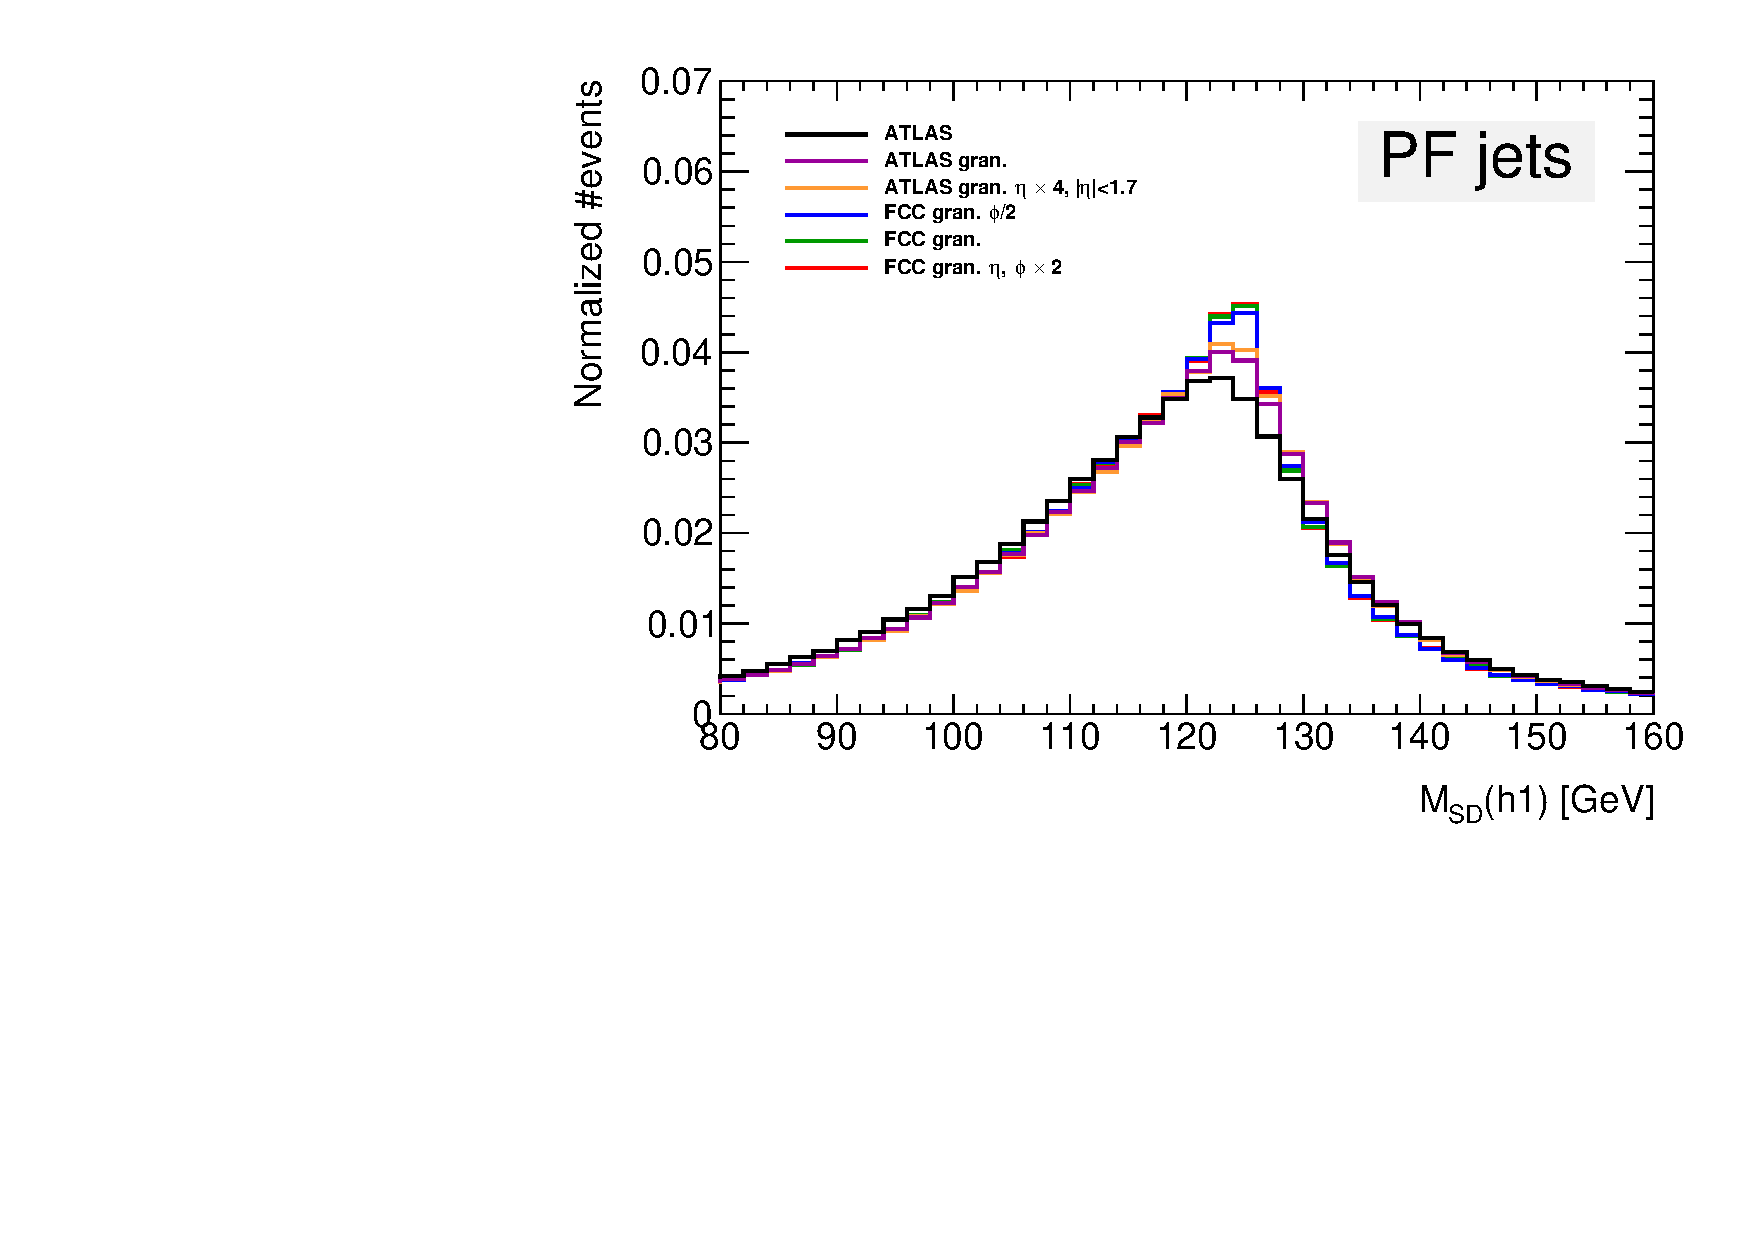
\includegraphics[trim={.65cm 0 0 0},clip,width=\linewidth]{./Figures/M.pdf}
		\label{fig:CompGran_M}
		%\caption{Leading Higgs candidate softdrop mass plot for the different detector configurations for the SM signal sample. This plot contains all the signal events that passed all the cuts of the baseline analysis. Note that the x axis range is from $80$ GeV to $160$ GeV in order to make the differences between the histograms more clear.}
	\end{minipage}%
	\begin{minipage}{.5\textwidth}
		\centering
		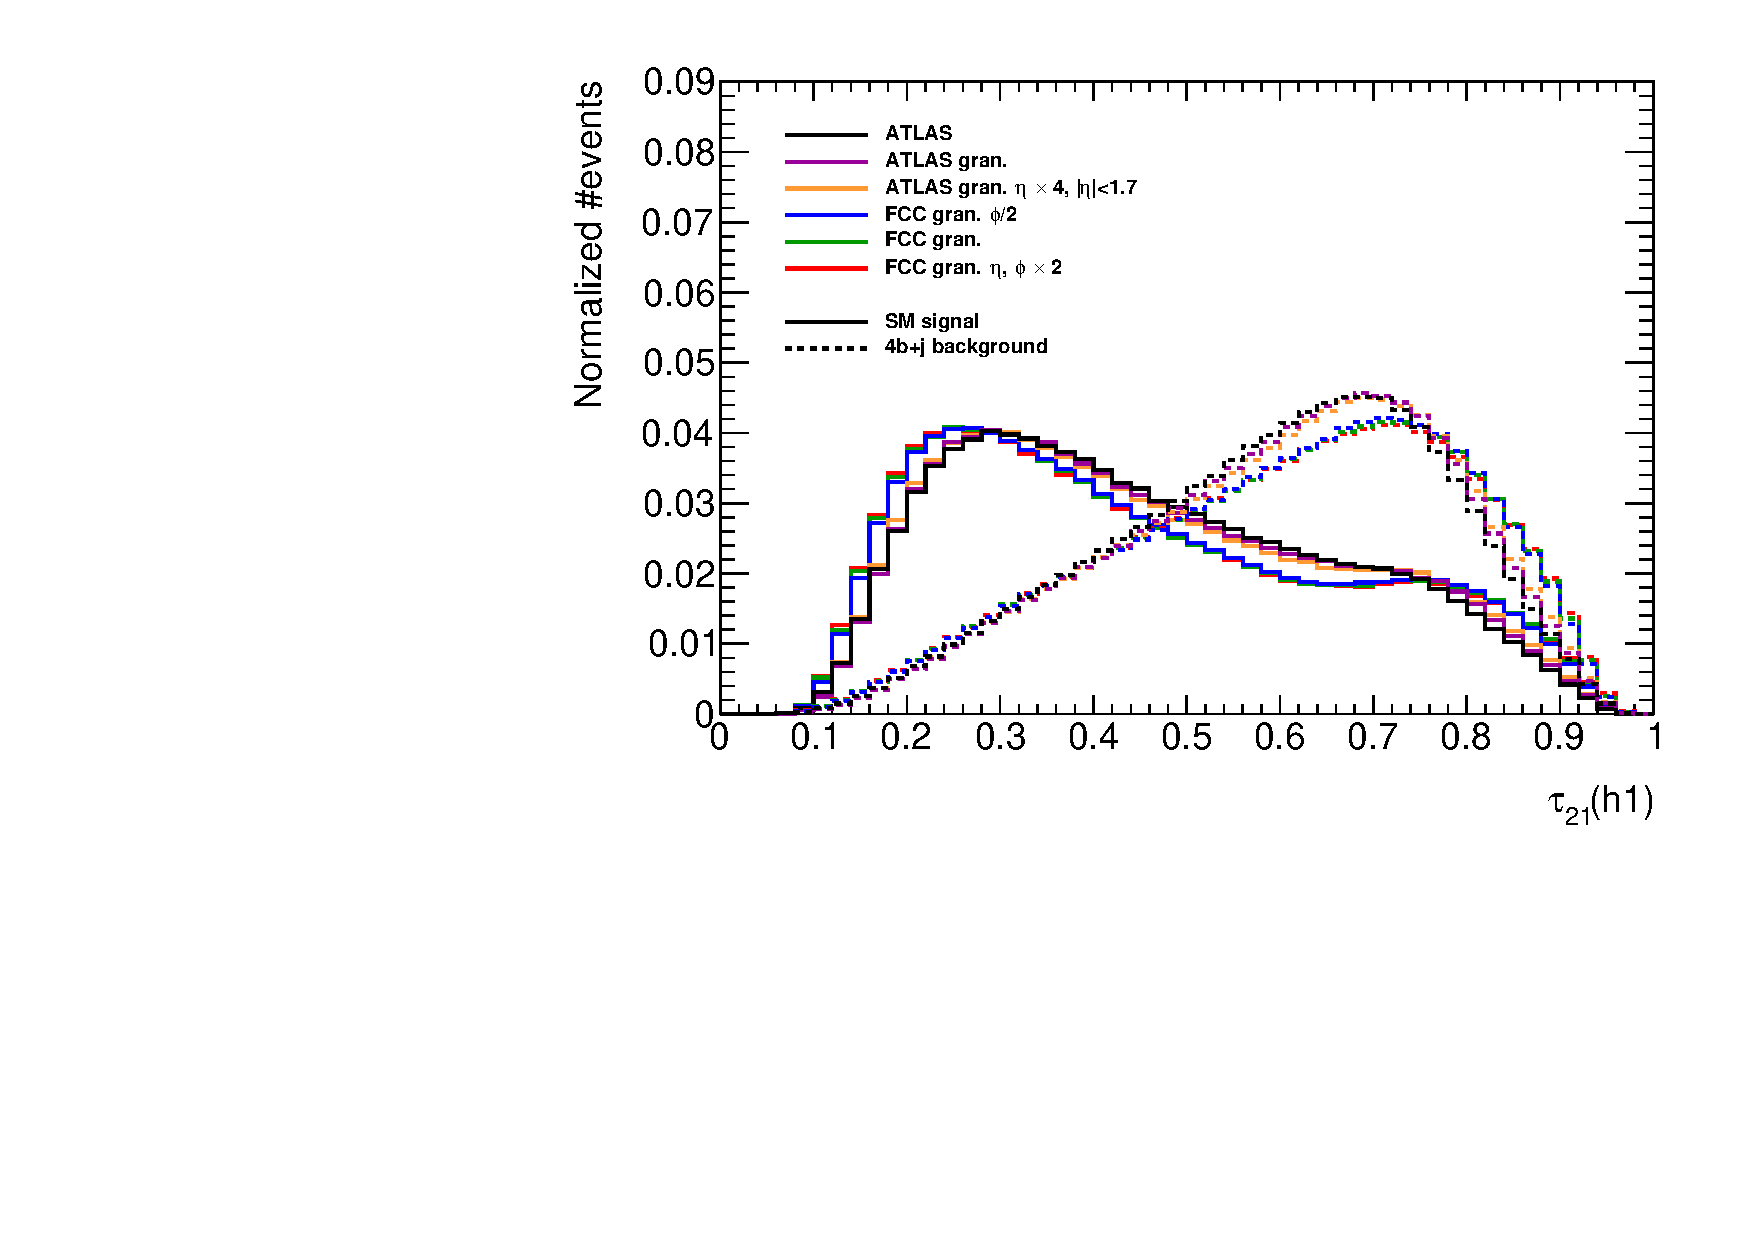
\includegraphics[trim={0 0 .65cm 0},clip,width=\linewidth]{./Figures/tau21.pdf}
		%\caption{Leading Higgs candidate $\tau_{21}$ plot for the different detector configurations for the SM signal sample. This plot contains all the signal events that passed all the cuts of the baseline analysis.}
		\label{fig:CompGran_tau21}
	\end{minipage}
	\label{fig:CompGran}
	\caption{Leading Higgs candidate softdrop mass (left) and $\tau_{21}$ (right) plots for the different detector configurations for the SM signal sample. The plots contain all the signal events that passed all the cuts of the baseline analysis. For the plot on the left note that the x axis range is from $80$ GeV to $160$ GeV in order to make the differences between the histograms more clear.}
\end{figure}

%\begin{figure}
%	\centering
%	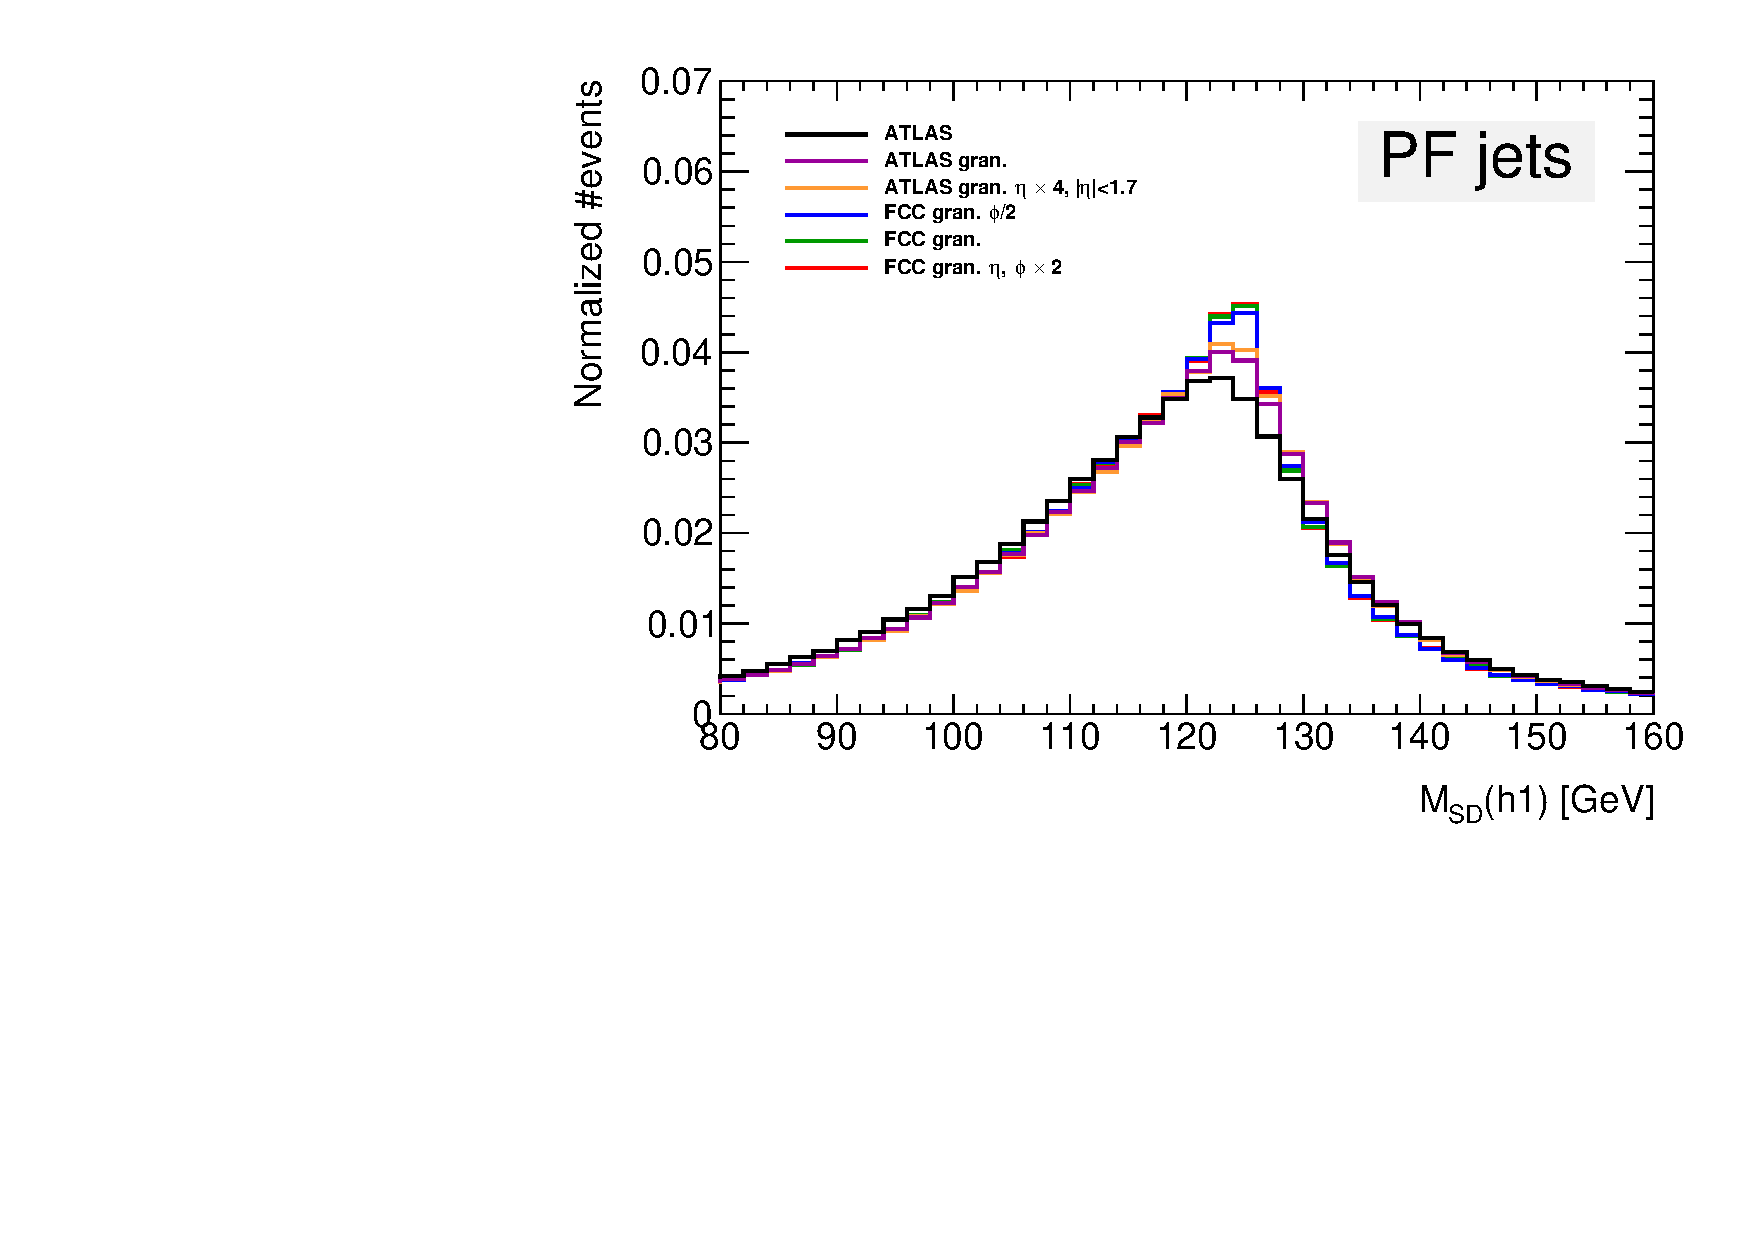
\includegraphics[width=\linewidth]{./Figures/M.pdf}
%	\label{fig:CompGran_M}
%	\caption{Leading Higgs candidate softdrop mass plot for the different detector configurations for the SM signal sample. This plot contains all the signal events that passed all the cuts of the baseline analysis. Note that the x axis range is from $80$ GeV to $160$ GeV in order to make the differences between the histograms more clear.}
%\end{figure}
%
%\begin{figure}
%	\centering
%	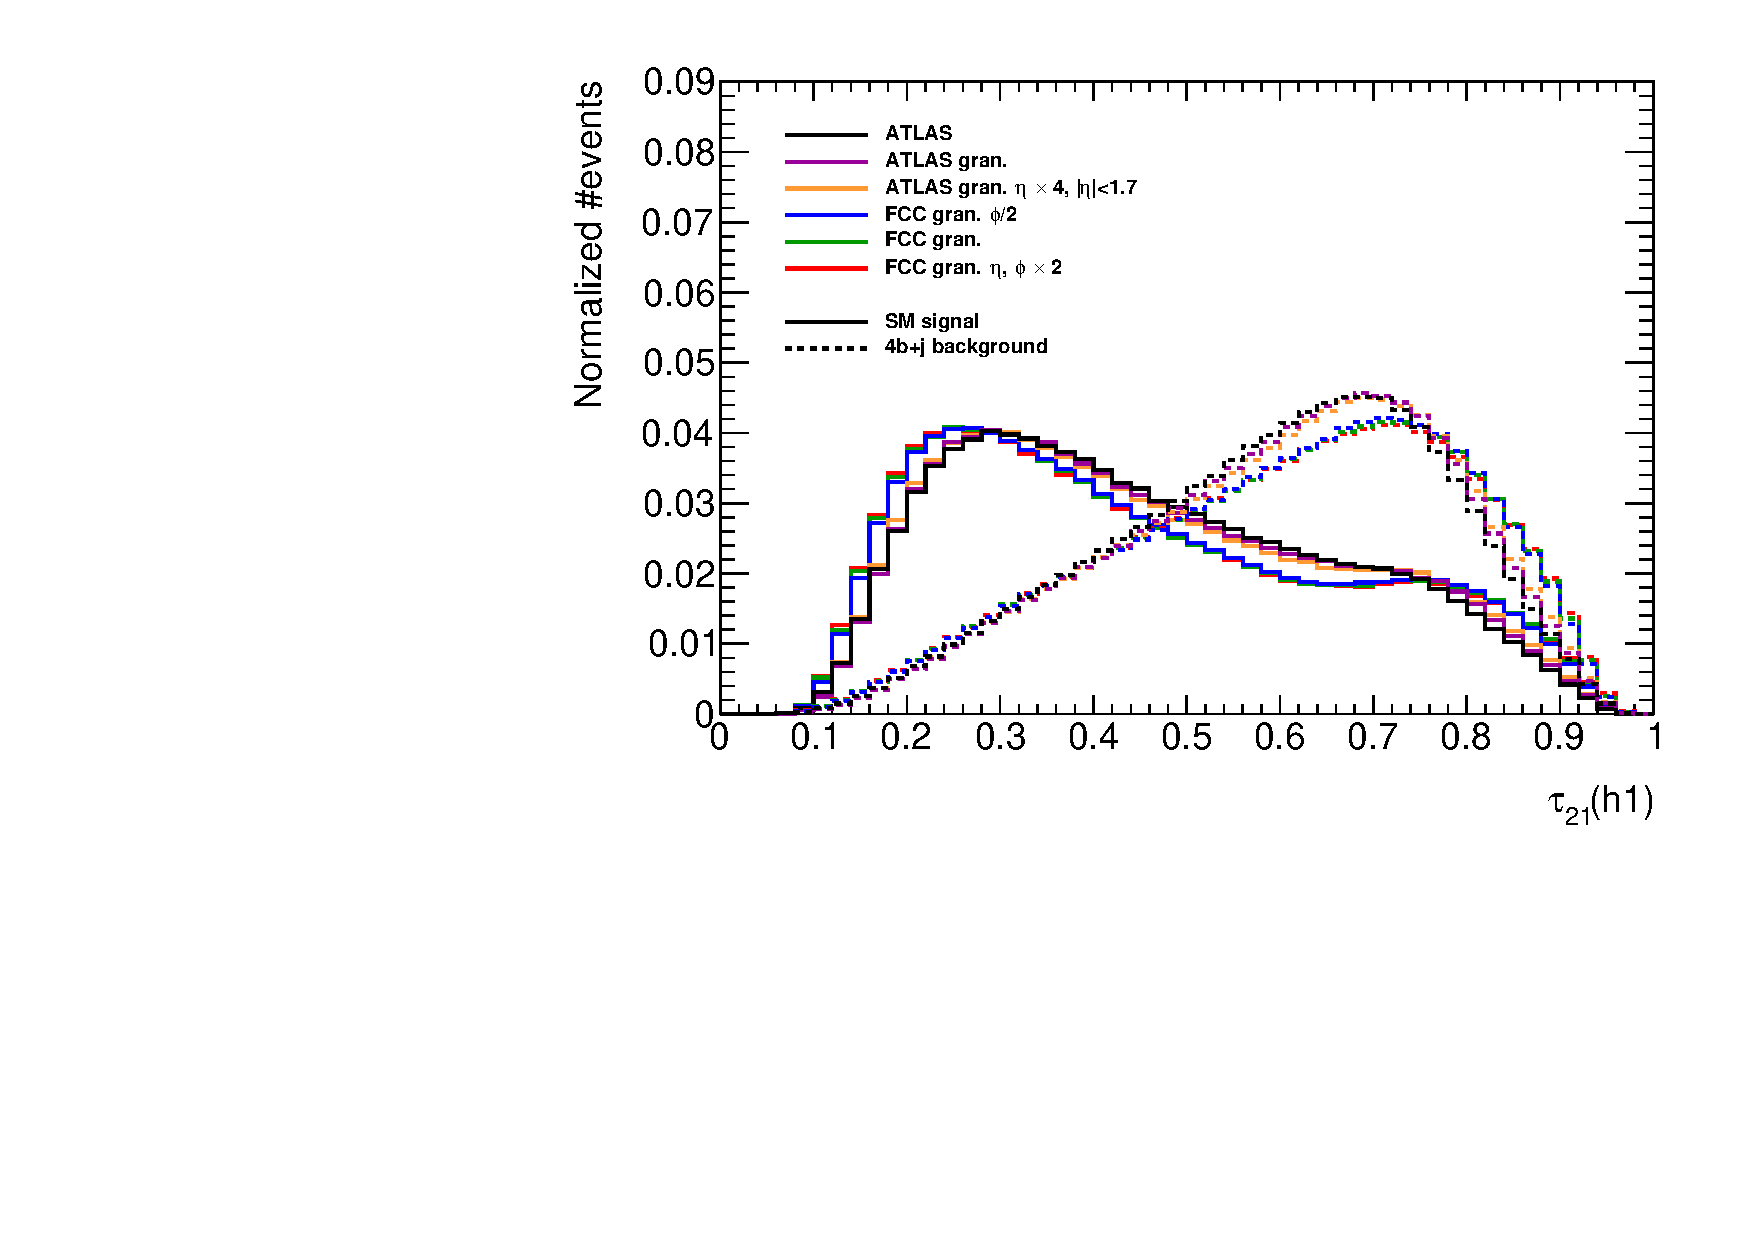
\includegraphics[width=\linewidth]{./Figures/tau21.pdf}
%	\label{fig:CompGran_tau21}
%	\caption{Leading Higgs candidate $\tau_{21}$ plot for the different detector configurations for the SM signal sample. This plot contains all the signal events that passed all the cuts of the baseline analysis.}
%\end{figure}

\begin{figure}
	\centering
	\begin{minipage}{.5\textwidth}
		\centering
		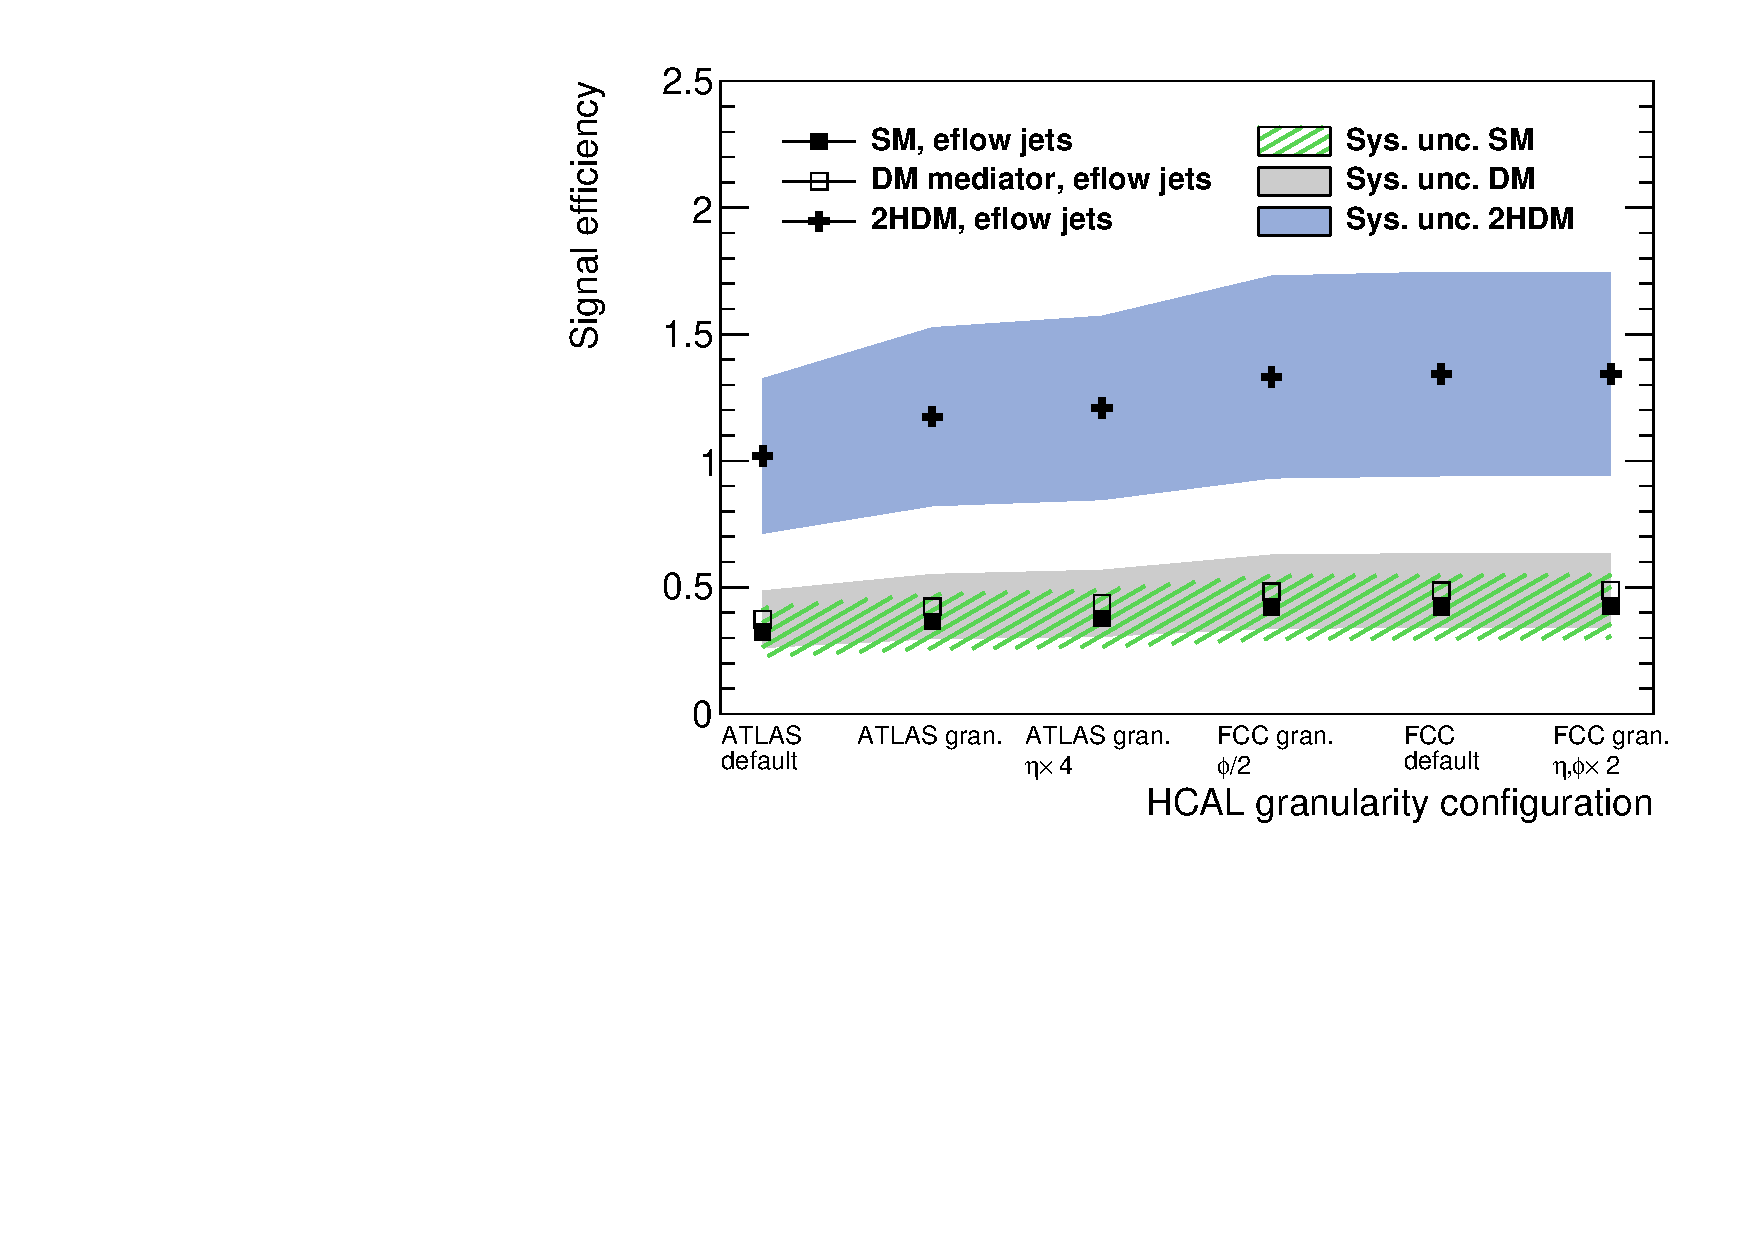
\includegraphics[trim={.6cm 0 0 0},clip,width=\linewidth]{./Figures/EffvsGran_PFjets.pdf}
	\end{minipage}%
	\begin{minipage}{.5\textwidth}
		\centering
		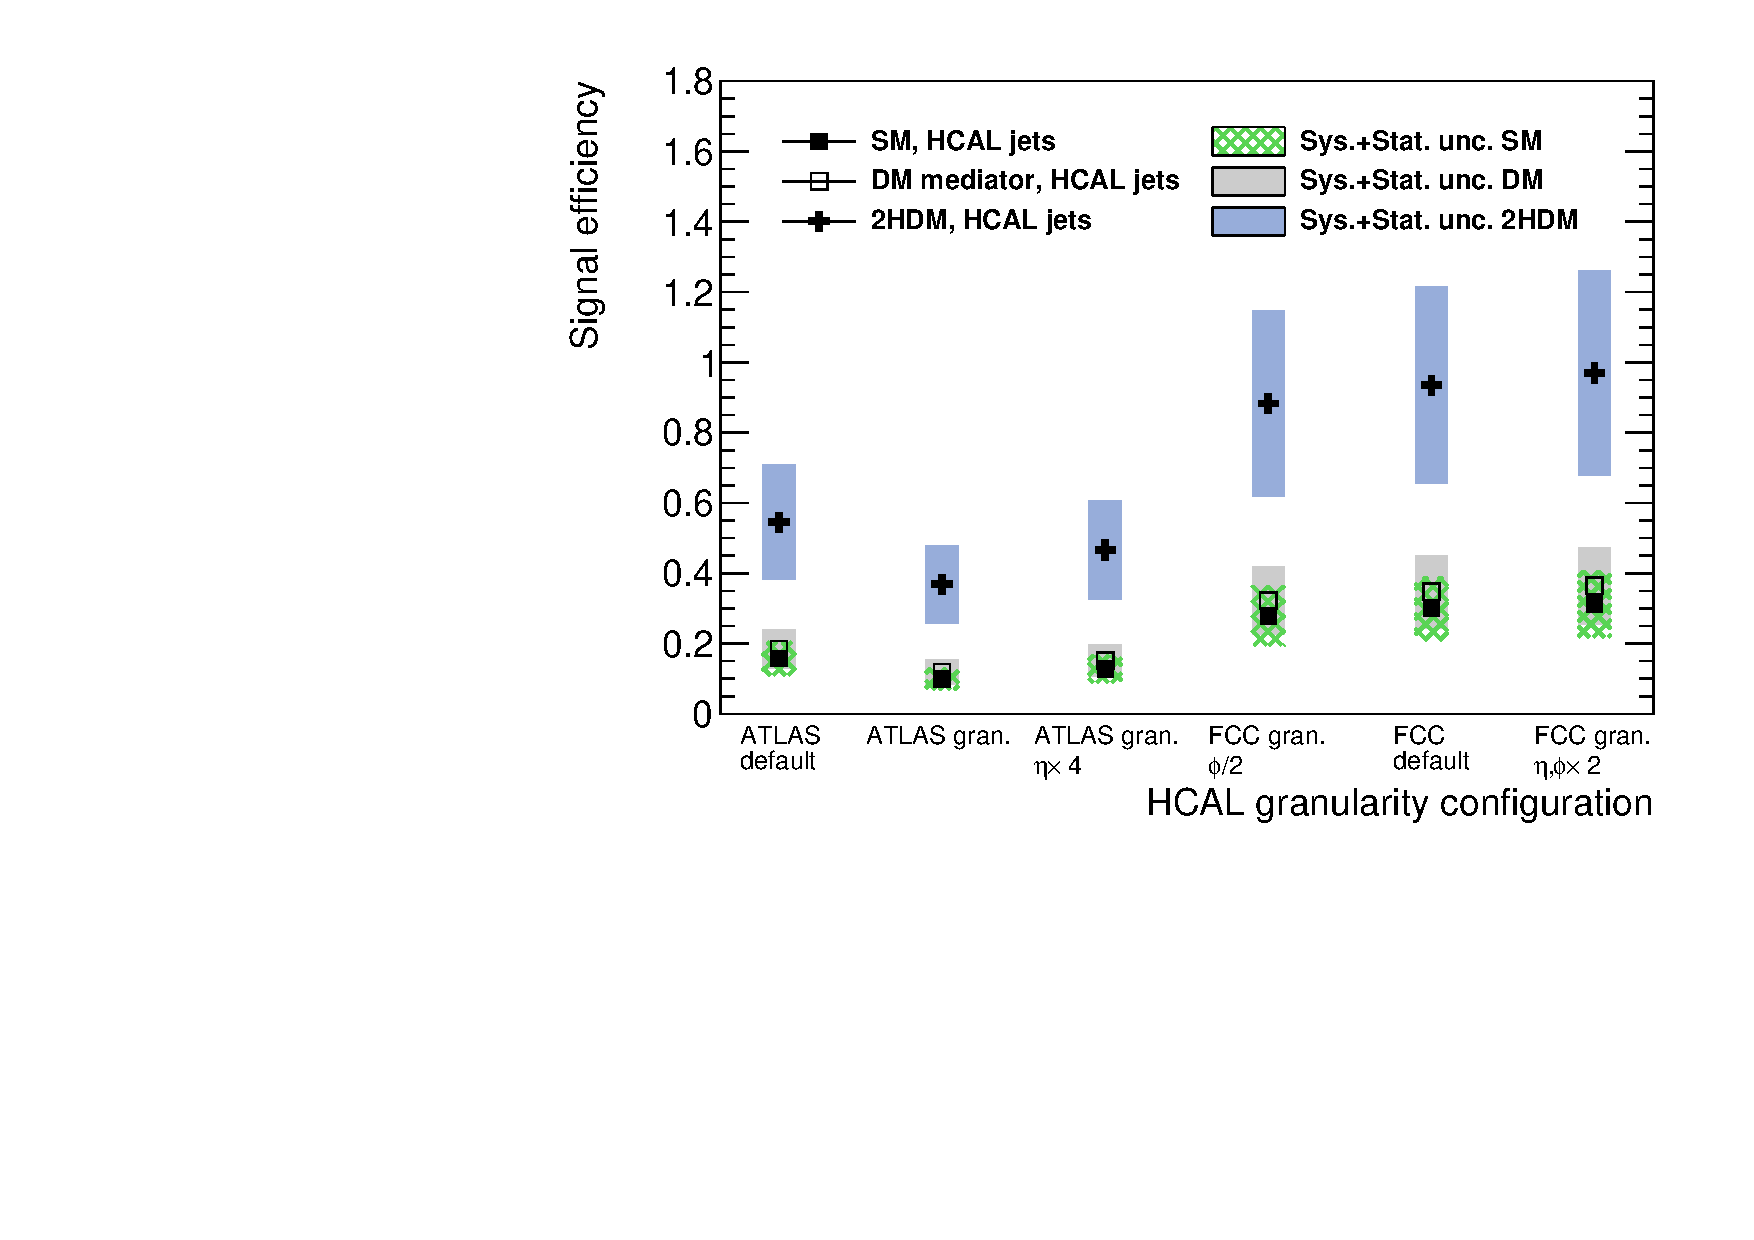
\includegraphics[trim={0 0 .6cm 0},clip,width=\linewidth]{./Figures/EffvsGran_CALOjets.pdf}
	\end{minipage}
	\label{fig:EffvsGran}
	\caption{Signal efficiency as a function of the detector configuration for particle flow jets (left) and pure calorimeter (HCAL) jets (right). Three signal models are shown: SM (filled squares), $1$ TeV DM mediator (empty squares) and type II 2HDM with $m_H=900$ GeV (crosses). The error bars are drawn but are smaller than the markers.}
\end{figure}

\begin{figure}
	\centering
	\begin{minipage}{.5\textwidth}
		\centering
		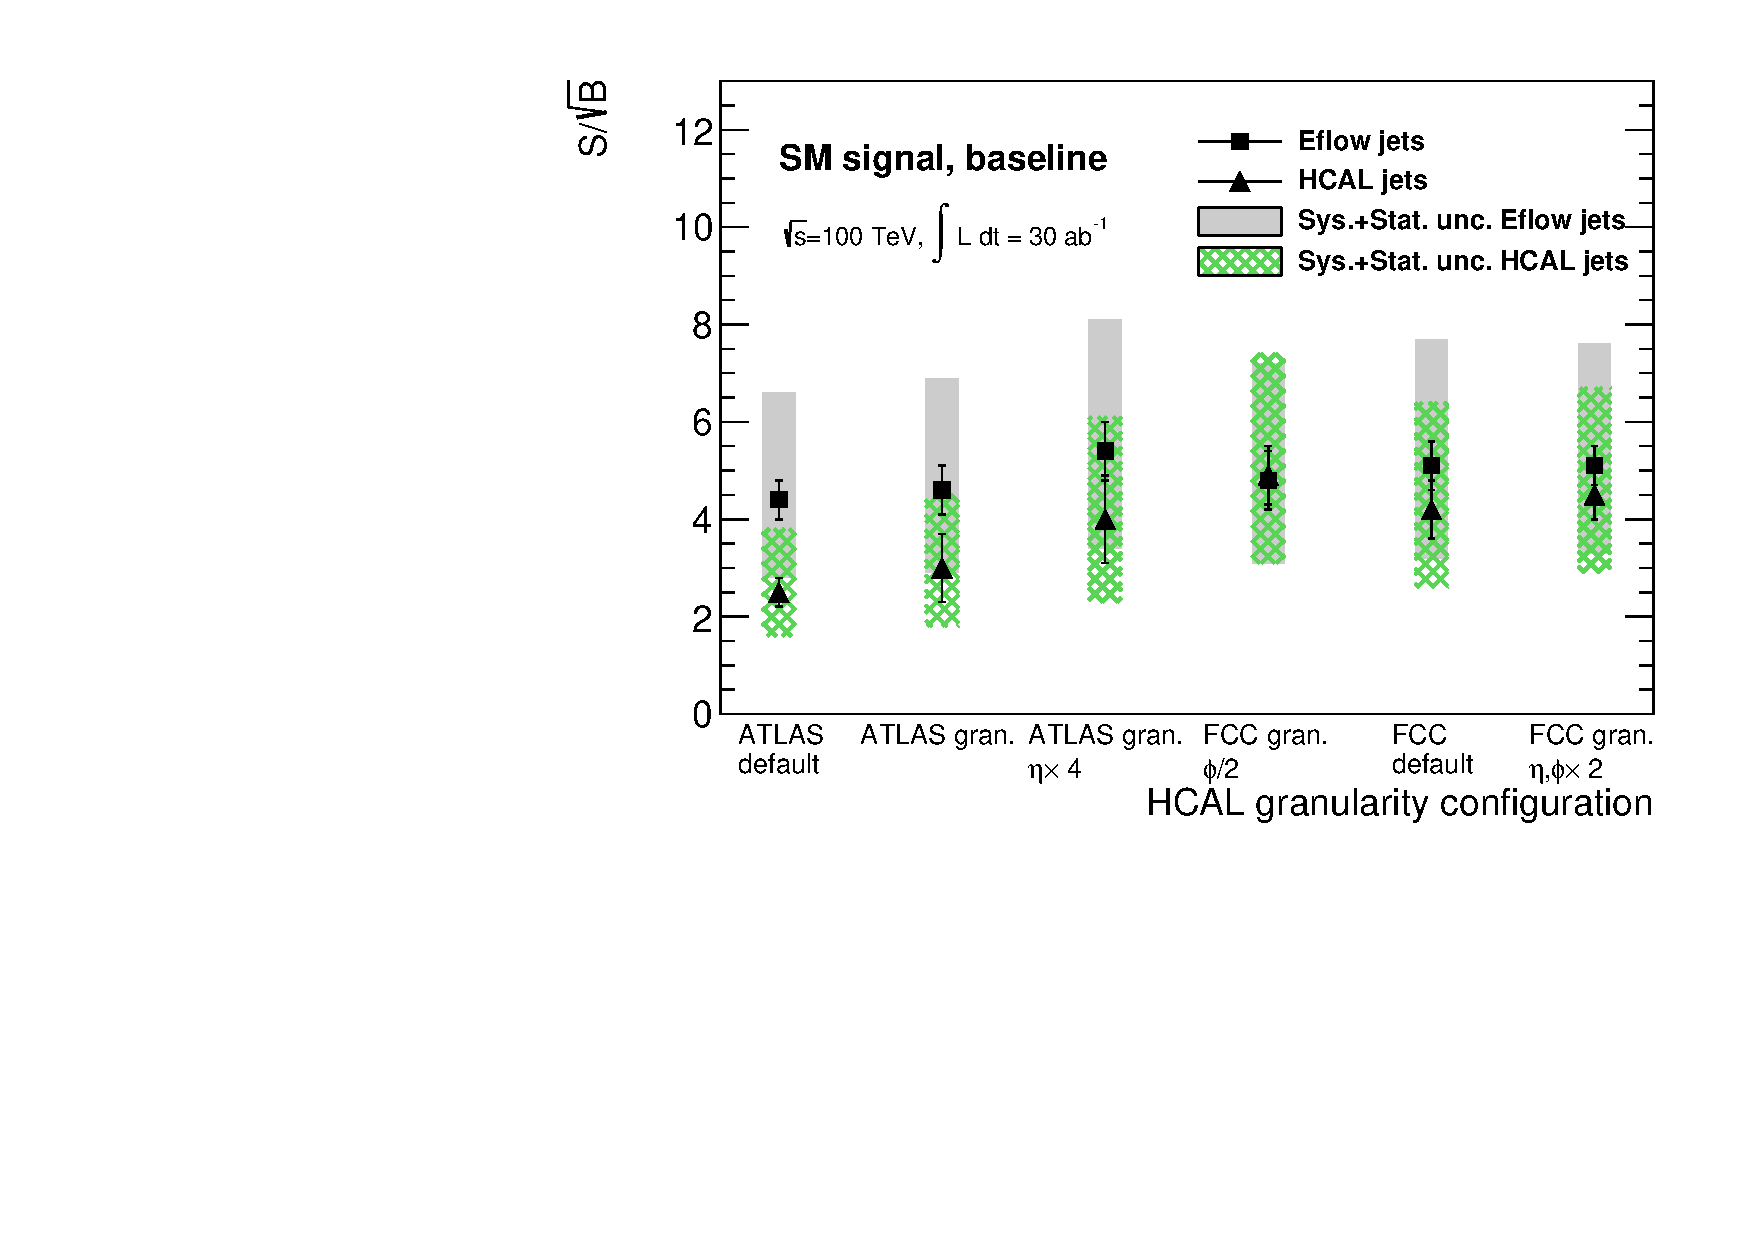
\includegraphics[trim={.6cm 0 0 0},clip,width=\linewidth]{./Figures/SSBvsGran_SM.pdf}
	\end{minipage}%
	\begin{minipage}{.5\textwidth}
		\centering
		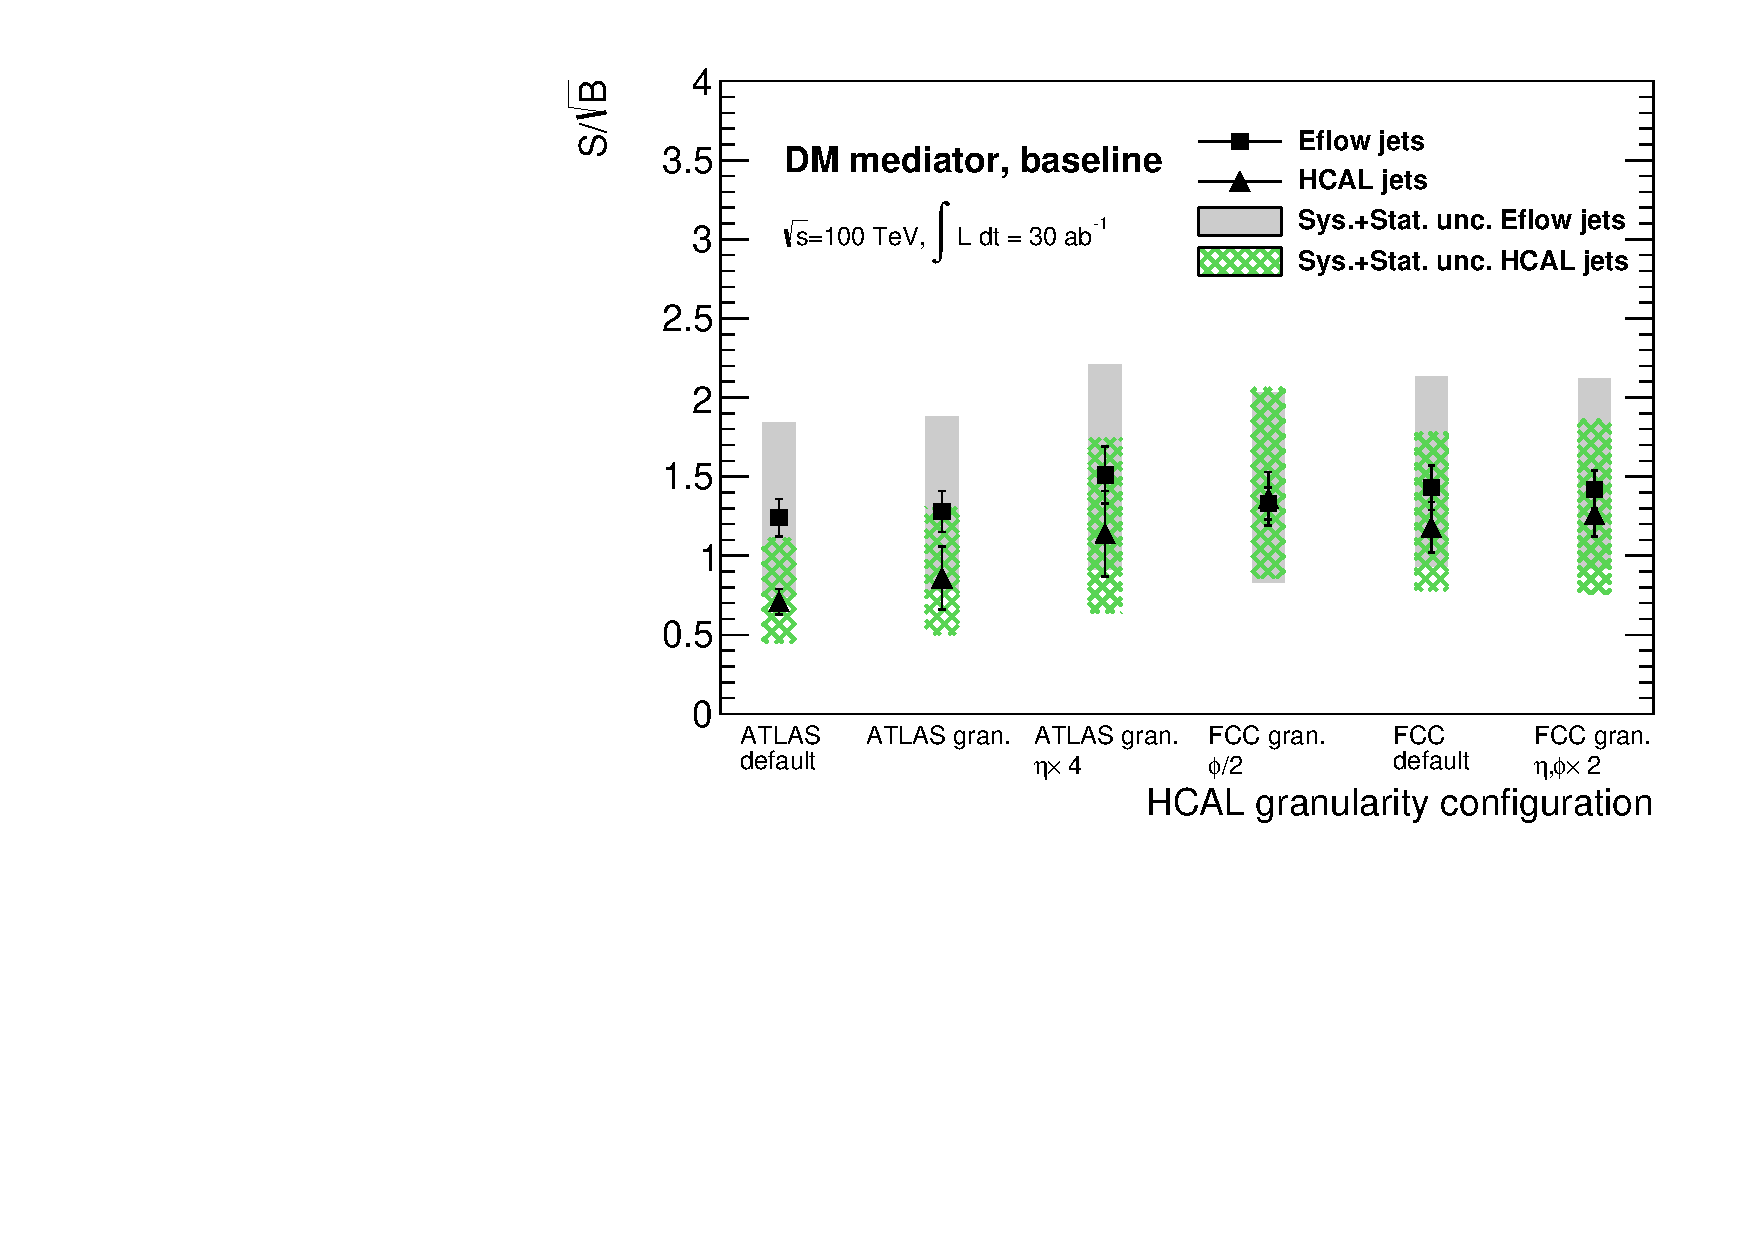
\includegraphics[trim={0 0 .6cm 0},clip,width=\linewidth]{./Figures/SSBvsGran_DM.pdf}
	\end{minipage}
	\label{fig:SSBvsGran1}
	\caption{Significance $(S/\sqrt{B})$ as a function of the detector configuration for $\mathcal{L}=30~\text{ab}^{-1}$ (filled) and $\mathcal{L}=3~\text{ab}^{-1}$ (empty) and for particle flow jets (squares) and pure calorimeter (HCAL) jets (triangles) for the SM signal model (left) and for the $1$ TeV DM mediator model (right).}
\end{figure}

\begin{figure}
	\centering
	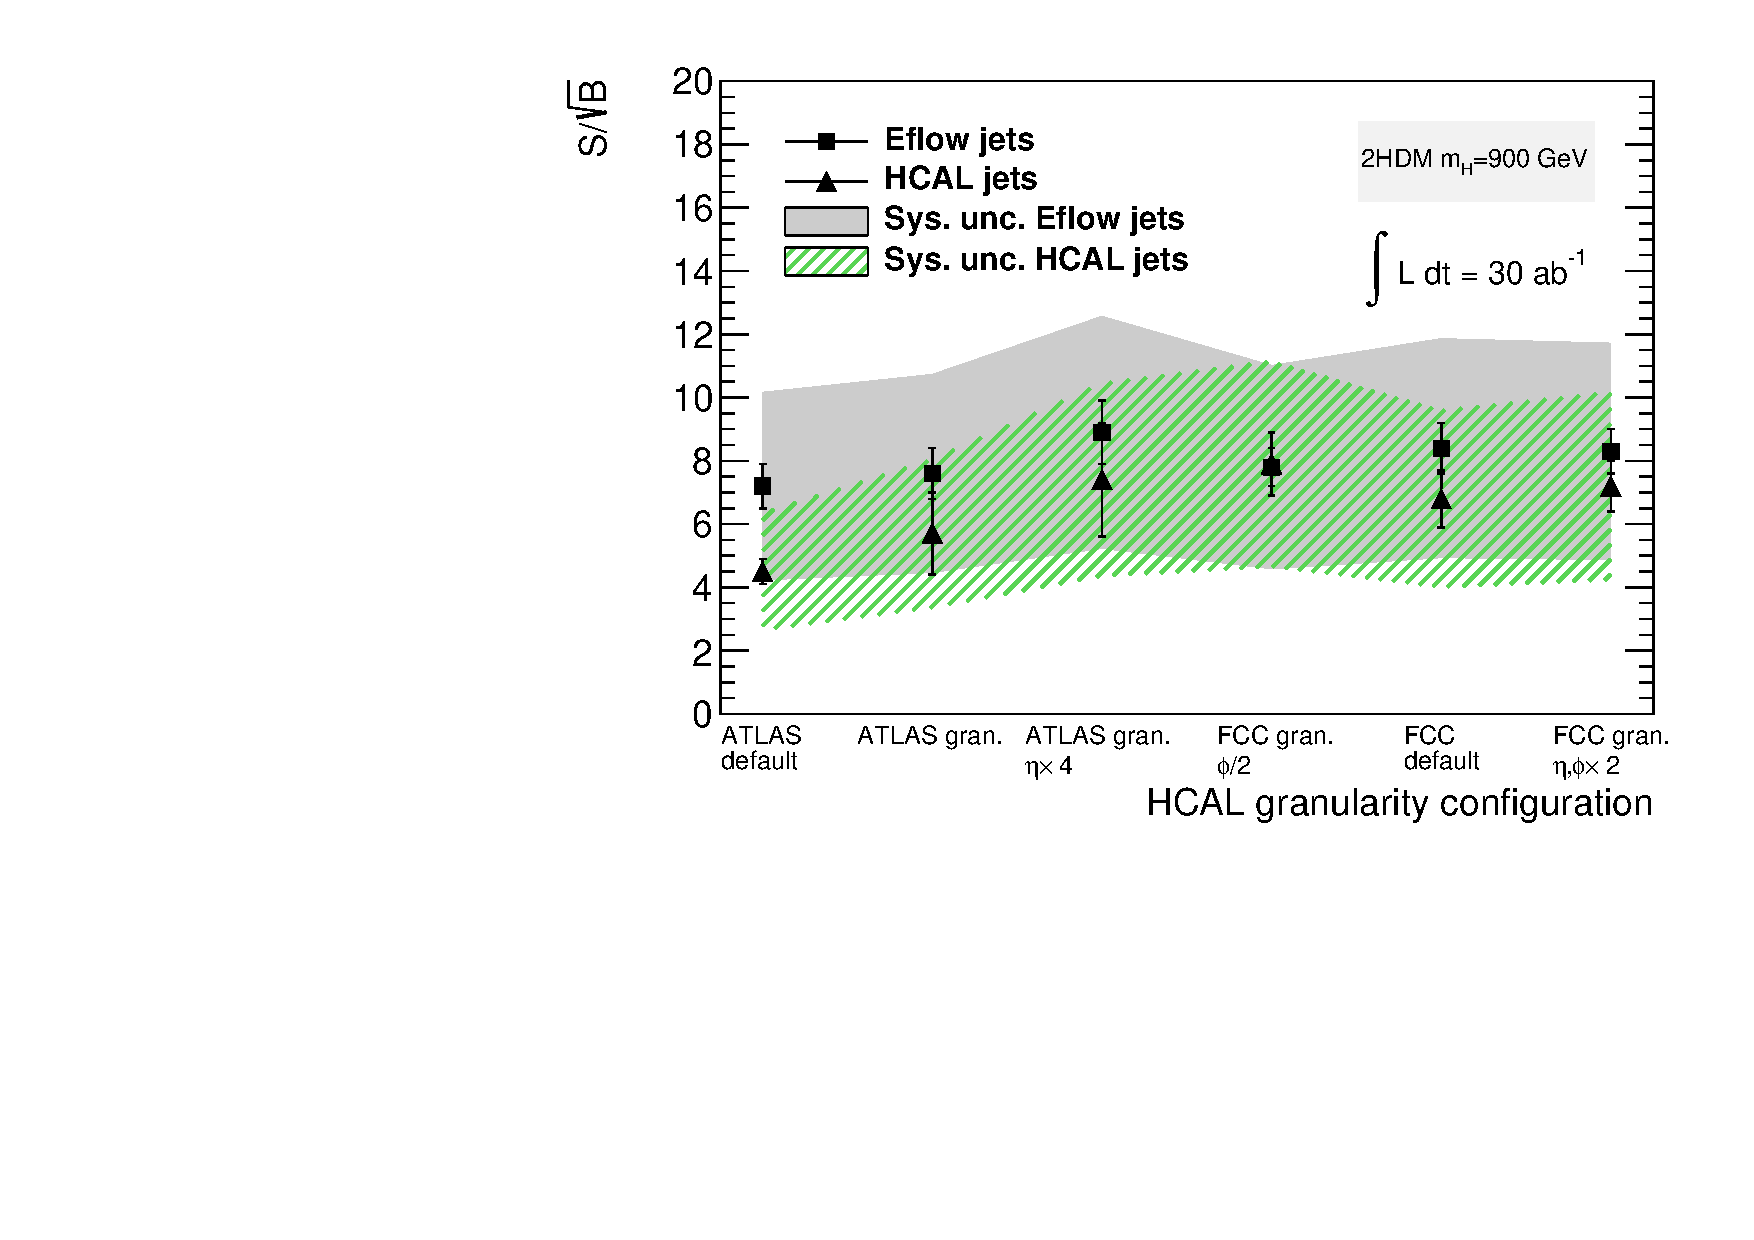
\includegraphics[width=0.5\linewidth]{./Figures/SSBvsGran_2HDM.pdf}
	\label{fig:SSBvsGran_2HDM}
	\caption{Significance $(S/\sqrt{B})$ as a function of the detector configuration for $\mathcal{L}=30~\text{ab}^{-1}$ (filled) and $\mathcal{L}=3~\text{ab}^{-1}$ (empty) and for particle flow jets (squares) and pure calorimeter (HCAL) jets (triangles) for the type II 2HDM with $m_H=900$ GeV.}
\end{figure}

%\begin{figure}[!htb]
%  \centering
%  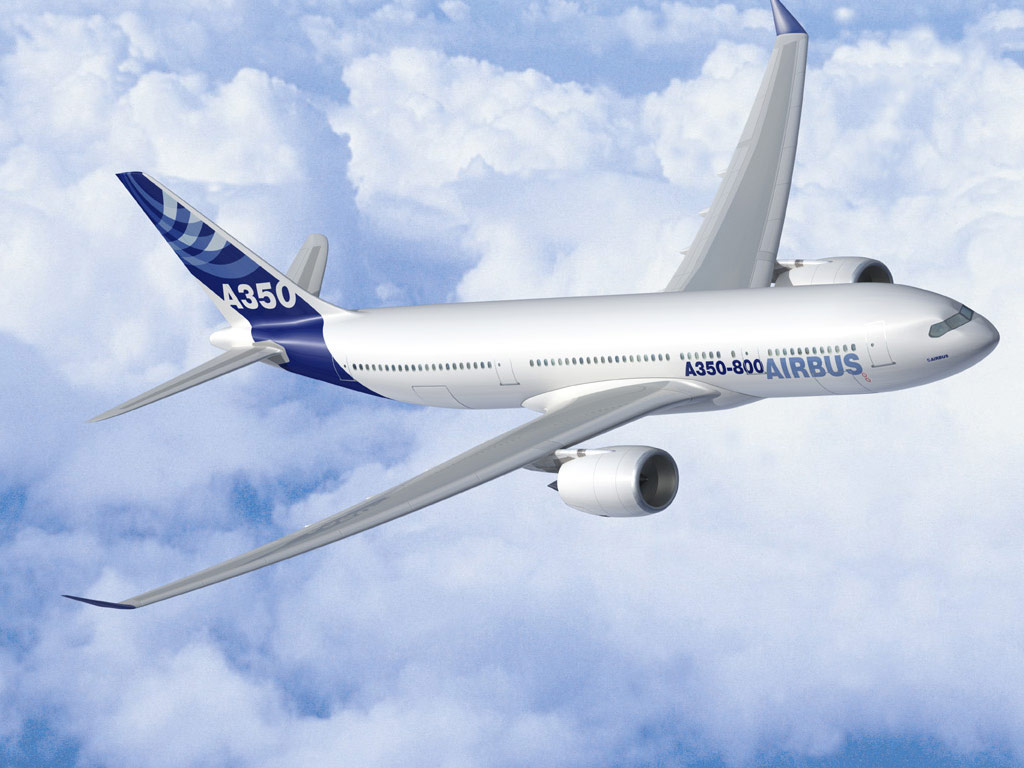
\includegraphics[width=0.25\textwidth]{Figures/Airbus_A350.jpg}
%  \caption[Caption for figure in TOC.]{Caption for figure.}
%  \label{fig:airbus1}
%\end{figure}
%
%\begin{figure}[!htb]
%  \begin{subfigmatrix}{2}
%    \subfigure[Airbus A320]{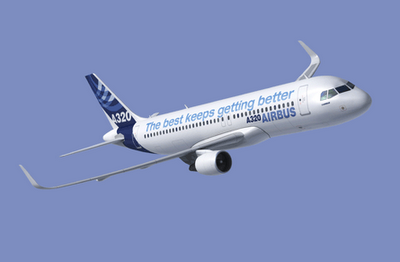
\includegraphics[width=0.49\linewidth]{Figures/Airbus_A320_sharklets.png}}
%    \subfigure[Bombardier CRJ200]{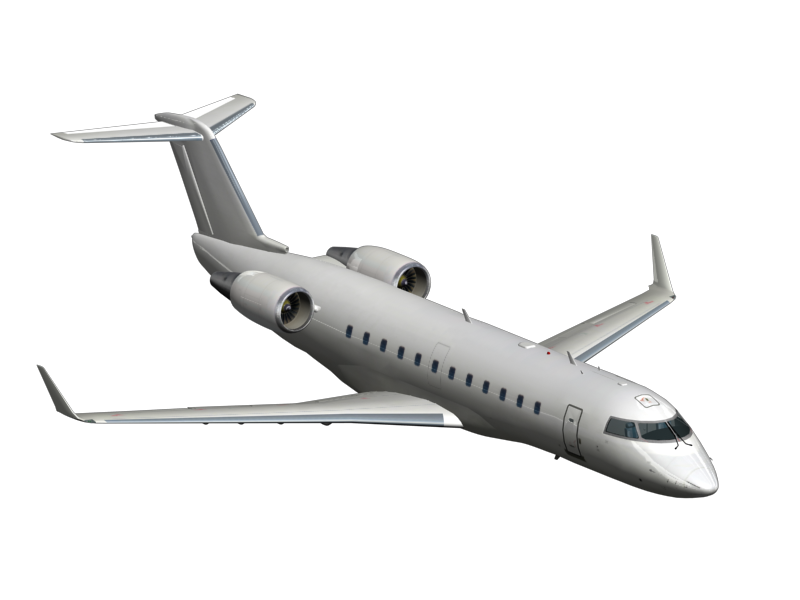
\includegraphics[width=0.49\linewidth]{Figures/Bombardier_CRJ200.png}}
%  \end{subfigmatrix}
%  \caption{Some aircrafts.}
%  \label{fig:aircrafts}
%\end{figure}
%
%Make reference to Figures \ref{fig:airbus1} and \ref{fig:aircrafts}.
%
%By default, the supported file types are {\it .png,.pdf,.jpg,.mps,.jpeg,.PNG,.PDF,.JPG,.JPEG}.
%
%See \url{http://mactex-wiki.tug.org/wiki/index.php/Graphics_inclusion} for adding support to other extensions.
%
%
%% ----------------------------------------------------------------------
%\subsubsection{Drawings}
%\label{subsection:drawings}
%
%Insert your subsection material and for instance a few drawings...
%
%The schematic illustrated in Fig.~\ref{fig:algorithm} can represent some sort of algorithm.
%
%\begin{figure}[!htb]
%  \centering
%  \scriptsize
%%  \footnotesize 
%%  \small
%  \setlength{\unitlength}{0.9cm}
%  \begin{picture}(8.5,6)
%    \linethickness{0.3mm}
%
%    \put(3,6){\vector(0,-1){1}}
%    \put(3.5,5.4){$\bf \alpha$}
%    \put(3,4.5){\oval(6,1){}}
%    %\put(0,4){\framebox(6,1){}}
%    \put(0.3,4.4){Grid Generation: \quad ${\bf x} = {\bf x}\left({\bf \alpha}\right)$}
%
%    \put(3,4){\vector(0,-1){1}}
%    \put(3.5,3.4){$\bf x$}
%    \put(3,2.5){\oval(6,1){}}
%    %\put(0,2){\framebox(6,1){}}
%    \put(0.3,2.4){Flow Solver: \quad ${\cal R}\left({\bf x},{\bf q}\left({\bf x}\right)\right) = 0$}
%
%    \put(6.0,2.5){\vector(1,0){1}}
%    \put(6.4,3){$Y_1$}
%
%    \put(3,2){\vector(0,-1){1}}
%    \put(3.5,1.4){$\bf q$}
%    \put(3,0.5){\oval(6,1){}}
%    %\put(0,0){\framebox(6,1){}}
%    \put(0.3,0.4){Structural Solver: \quad ${\cal M}\left({\bf x},{\bf q}\left({\bf x}\right)\right) = 0$}
%
%    \put(6.0,0.5){\vector(1,0){1}}
%    \put(6.4,1){$Y_2$}
%
%    %\put(7.8,2.5){\oval(1.6,5){}}
%    \put(7.0,0){\framebox(1.6,5){}}
%    \put(7.1,2.5){Optimizer}
%    \put(7.8,5){\line(0,1){1}}
%    \put(7.8,6){\line(-1,0){4.8}}
%  \end{picture}
%  \caption{Schematic of some algorithm.}
%  \label{fig:algorithm}
%\end{figure}
%
%
%% ----------------------------------------------------------------------
%\subsection{Equations}
%\label{subsection:equations}
%
%Equations can be inserted in different ways.
%
%The simplest way is in a separate line like this
%
%\begin{equation}
%  \frac{{\rm d} q_{ijk}}{{\rm d} t} + {\cal R}_{ijk}({\bf q}) = 0 \,.
%\label{eq:ode}
%\end{equation}
%
%If the equation is to be embedded in the text. One can do it like this ${\partial {\cal R}}/{\partial {\bf q}}=0$.
%
%It may also be split in different lines like this
%
%\begin{eqnarray}
%  {\rm Minimize}   && Y({\bf \alpha},{\bf q}({\bf \alpha}))            \nonumber           \\
%  {\rm w.r.t.}     && {\bf \alpha} \,,                                 \label{eq:minimize} \\
%  {\rm subject~to} && {\cal R}({\bf \alpha},{\bf q}({\bf \alpha})) = 0 \nonumber           \\
%                   &&       C ({\bf \alpha},{\bf q}({\bf \alpha})) = 0 \,. \nonumber
%\end{eqnarray}
%
%It is also possible to use subequations. Equations~\ref{eq:continuity}, \ref{eq:momentum} and \ref{eq:energy} form the Naver--Stokes equations~\ref{eq:NavierStokes}.
%
%\begin{subequations}
%    \begin{equation}
%    \frac{\partial \rho}{\partial t} + \frac{\partial}{\partial x_j}\left( \rho u_j \right) = 0 \,,
%    \label{eq:continuity}
%    \end{equation}
%    \begin{equation}
%    \frac{\partial}{\partial t}\left( \rho u_i \right) + \frac{\partial}{\partial x_j} \left( \rho u_i u_j + p \delta_{ij} - \tau_{ji} \right) = 0, \quad i=1,2,3 \,,
%    \label{eq:momentum}
%    \end{equation}
%    \begin{equation}
%        \frac{\partial}{\partial t}\left( \rho E \right) + \frac{\partial}{\partial x_j} \left( \rho E u_j + p u_j - u_i \tau_{ij} + q_j \right) = 0 \,.
%    \label{eq:energy}
%    \end{equation}
%\label{eq:NavierStokes}%
%\end{subequations}
%
%
%% ----------------------------------------------------------------------
%\subsection{Tables}
%\label{section:tables}
%
%Insert your subsection material and for instance a few tables...
%
%Make sure all tables presented are referenced in the text!
%
%Follow some guidelines when making tables:
%
%\begin{itemize}
%  \item Avoid vertical lines
%  \item Avoid “boxing up” cells, usually 3 horizontal lines are enough: above, below, and after heading
%  \item Avoid double horizontal lines
%  \item Add enough space between rows
%\end{itemize}
%
%\begin{table}[!htb]
%  \renewcommand{\arraystretch}{1.2} % more space between rows
%  \centering
%  \begin{tabular}{lccc}
%    \toprule
%    Model           & $C_L$ & $C_D$ & $C_{M y}$ \\
%    \midrule
%    Euler           & 0.083 & 0.021 & -0.110    \\
%    Navier--Stokes  & 0.078 & 0.023 & -0.101    \\
%    \bottomrule
%  \end{tabular}
%  \caption[Table caption shown in TOC.]{Table caption.}
%  \label{tab:aeroCoeff}
%\end{table}
%
%Make reference to Table \ref{tab:aeroCoeff}.
%
%Tables \ref{tab:memory} and \ref{tab:multipleColumns} are examples of tables with merging columns:
%
%\begin{table}[!htb]
%  \renewcommand{\arraystretch}{1.2} % more space between rows
%  \centering
%  \begin{tabular}[]{lrr}
%    \toprule
%                & \multicolumn{2}{c}{\underline{Virtual memory [MB]}} \\
%                & Euler       & Navier--Stokes \\
%    \midrule
%      Wing only &  1,000      &    2,000       \\
%      Aircraft  &  5,000      &   10,000       \\
%      (ratio)   & $5.0\times$ & $5.0\times$    \\
%    \bottomrule
%  \end{tabular}
%  \caption{Memory usage comparison (in MB).}
%  \label{tab:memory}
%\end{table}
%
%\begin{table}[!htb]
%  \centering
%  \renewcommand{\arraystretch}{1.2} % more space between rows
%  \begin{tabular}{@{}rrrrcrrr@{}} % remove space to the vertical edges @{}...@{}
%    \toprule
%      & \multicolumn{3}{c}{$w = 2$} & \phantom{abc} & \multicolumn{3}{c}{$w = 4$} \\
%    \cmidrule{2-4}
%    \cmidrule{6-8}
%      & $t=0$ & $t=1$ & $t=2$ && $t=0$ & $t=1$ & $t=2$ \\
%    \midrule
%      $dir=1$
%      \\
%      $c$ &  0.07 &  0.16 &  0.29 &&  0.36 &  0.71 &   3.18 \\
%      $c$ & -0.86 & 50.04 &  5.93 && -9.07 & 29.09 &  46.21 \\
%      $c$ & 14.27 &-50.96 &-14.27 && 12.22 &-63.54 &-381.09 \\
%      $dir=0$
%      \\
%      $c$ &  0.03 &  1.24 &  0.21 &&  0.35 & -0.27 &  2.14 \\
%      $c$ &-17.90 &-37.11 &  8.85 &&-30.73 & -9.59 & -3.00 \\
%      $c$ &105.55 & 23.11 &-94.73 &&100.24 & 41.27 &-25.73 \\
%    \bottomrule
%  \end{tabular}
%  \caption{Another table caption.}
%  \label{tab:multipleColumns}
%\end{table}
%
%An example with merging rows can be seen in Tab.\ref{tab:multipleRows}.
%
%\begin{table}[!htb]
%  \renewcommand{\arraystretch}{1.2} % more space between rows
%  \centering
%  \begin{tabular}{ccccc}
%    \toprule
%      \multirow{2}{*}{ABC} & \multicolumn{4}{c}{header} \\
%      \cmidrule{2-5} & 1.1 & 2.2 & 3.3 & 4.4 \\
%    \midrule
%      \multirow{2}{*}{IJK} & \multicolumn{2}{c}{\multirow{2}{*}{group}} & 0.5 & 0.6 \\
%      \cmidrule{4-5}       & \multicolumn{2}{c}{}                       & 0.7 & 1.2 \\
%    \bottomrule
%  \end{tabular}
%  \caption{Yet another table caption.}
%  \label{tab:multipleRows}
%\end{table}
%
%If the table has too many columns, it can be scaled to fit the text widht, as in Tab.\ref{tab:scale}.
%\begin{table}[!htb]
%  \renewcommand{\arraystretch}{1.2} % more space between rows
%  \centering
%  \resizebox*{\textwidth}{!}{%
%    \begin{tabular}[]{lcccccccccc}
%      \toprule
%        Variable &  a  &  b  &  c  &  d  &  e  &  f  &  g  &  h  &  i  &  j  \\
%      \midrule
%        Test 1   &  10,000 &  20,000 &  30,000 &  40,000 &  50,000 &  60,000 &  70,000 &  80,000 &  90,000 & 100,000 \\
%        Test 2   &  20,000 &  40,000 &  60,000 &  80,000 & 100,000 & 120,000 & 140,000 & 160,000 & 180,000 & 200,000 \\
%      \bottomrule
%    \end{tabular}
%  }%
%  \caption{Very wide table.}
%  \label{tab:scale}%
%\end{table}
%
%
%% ----------------------------------------------------------------------
%\subsection{Mixing}
%\label{section:mixing}
%
%If necessary, a figure and a table can be put side-by-side as in Fig.\ref{fig:side_by_side}
%
%\begin{figure}[!htb]
%  \begin{minipage}[b]{0.60\linewidth}
%    \centering
%    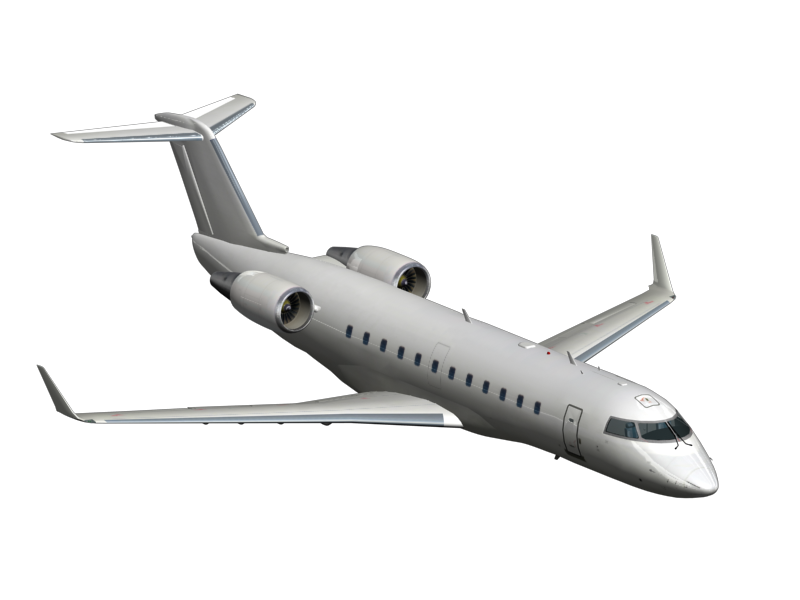
\includegraphics[width=\linewidth]{Figures/Bombardier_CRJ200}
%  \end{minipage}%
%  \begin{minipage}[b]{0.30\linewidth}
%    \centering
%    \begin{tabular}[b]{lll}
%      \toprule
%        \multicolumn{3}{c}{Legend} \\
%      \midrule
%        A & B & C \\
%        0 & 0 & 0 \\
%        0 & 1 & 0 \\
%        1 & 0 & 0 \\
%        1 & 1 & 1 \\
%      \bottomrule
%    \end{tabular}
%    \vspace{5em}
%  \end{minipage}
%\caption{Figure and table side-by-side.}
%\label{fig:side_by_side}
%\end{figure}

